\documentclass{beamer}

\beamertemplatenavigationsymbolsempty

\mode<presentation>
{
  \usetheme{default}
}

\usepackage[english]{babel}
\usepackage[latin1]{inputenc}
\usepackage{bussproofs}
\usepackage[retainorgcmds]{IEEEtrantools}

% needs debian package texlive-math-extra
\usepackage{stmaryrd} % for \llbracket, \rrbracket

\usepackage{times}
\usepackage[T1]{fontenc}
% Or whatever. Note that the encoding and the font should match. If T1
% does not look nice, try deleting the line with the fontenc.

\usepackage{tikz}
\usetikzlibrary{positioning}
\usetikzlibrary{calc}
\usetikzlibrary{matrix}

\title
{A Back End for SPL, the Simple Programming Language}

\author
{Markus~Klinik}

\institute[Radboud University Nijmegen]
{
  Radboud University Nijmegen
}

\date
{Compiler Construction 2013}


\newcommand{\arr}{\rightarrow}
\newcommand{\Arr}{\Rightarrow}
\newcommand{\semantics}[1]{\llbracket #1 \rrbracket}
\newcommand{\semanticsFd}[1]{\semantics{#1}_{F\delta}}

\begin{document}

\begin{frame}
  \titlepage
\end{frame}

\begin{frame}{Features}

  \begin{itemize}%[<+->]
    \item Every object occupies one machine word
    \item Polymorphic functions
    \item Poor man's higher-order functions
  \end{itemize}

\end{frame}

\begin{frame}{Meta}

  \begin{itemize}
    \item Implementation language: Haskell
    \item Time to implement: 35 hours
    \item Lines of code: 420
  \end{itemize}

\end{frame}

\begin{frame}[fragile]{Tuples and Lists}

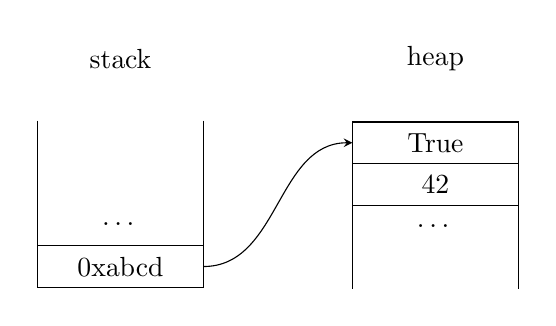
\begin{tikzpicture}

  \matrix (stack) [matrix of nodes
    , nodes={ minimum height = 1.5em
            , minimum width = 6em
            , outer sep = 0pt
            }
    , nodes in empty cells]
  {
    stack \\
    \\
    \\
    \\
    \ldots \\
    |[draw] (address) | 0xabcd \\
  };

  \draw (stack-3-1.north west) -- (stack-5-1.south west);
  \draw (stack-3-1.north east) -- (stack-5-1.south east);


  \matrix at (4,0) (heap) [matrix of nodes
    , nodes={ minimum height = 1.5em
            , minimum width = 6em
            , outer sep = 0pt
            }
    , nodes in empty cells]
  {
    heap \\
    \\
    |[draw] (true)| True \\
    |(42)| 42 \\
    \ldots \\
    \\
  };

  \draw (42.south west) -- (42.south east);

  \draw (true.north west) -- (heap-6-1.south west);
  \draw (true.north east) -- (heap-6-1.south east);

  \draw [>=stealth,->] (address.east) to [out=0,in=180] (true.west);

\end{tikzpicture}

\end{frame}


\end{document}
